
\chapter{Search problems} \label{chap:search_problems}

\section{Decision vs. Search}

For many years, the study of \textbf{decision problems} has been the main focus of computability theory. These problems can be described as simple questions with a \say{yes} or \say{no} answer, such as asking if some input object has some property or not. Each decision problem can be described as a subset of a given language $\Sigma^*$, where a string $\abk{o}$ that encodes an object $o$ is in the subset if and only if the answer to the problem for that object is positive. Usually, a positive \say{yes} answer is represented by a 1, while a negative \say{no} answer is represented by a 0. For example, given the language $\N$, the question \say{is $n$ a prime number?} is modeled by the decision problem $\mathrm{PRIMES} = \{n \in \N \mid n \text{ is prime}\}$.

\begin{definition}
 A decision problem for a property $P$ is a subset $L$ of a language $\Sigma^*$ such that $L = \{x \in \Sigma^* \mid P(x) = 1\}$.
\end{definition}

Any decidable problem can be \textit{decided} by a Turing machine, meaning that for any input $x$ of the language $\Sigma^*$ the \TM is capable of returning the answer 0 or 1. Decidability theory plays a core role in math and computer science since most problems can be modeled through it. However, by their nature, decision problems are limited. Some problems require a more complex result than a simple yes-or-no answer. Instead of asking the question \say{does this object have the required property?}, we may be more interested in the question \say{what gives this object the following property?}. These kinds of questions are modeled by \textbf{functional problems}, i.e. any problem where an output that is more complex than a yes-or-no answer is expected for a given input. Functional problems are "harder" types of problems, describing any possible type of computation achievable through the concept of computable function, even decidability itself (any decision problem is just a functional problem with only two possible outputs).

Formally, functional problems are described through the concept of relation: given a set of inputs $X$ and a set of possible outputs $Y$, a functional problem is as a relation $R \subseteq X \times Y$ such that the pair $(x,y)$ is in $R$ if and only if $y$ is the output to the input $x$ for the given question.

For example, the question \say{what is the prime factorization of $n$?} is modeled by the functional problem $\mathrm{FACTORING} = \{(n, (p_1, \ldots, p_k)) \in \N \times \N^k \mid n = p_1 \cdot \ldots \cdot p_k\}$.

We observe that questions like \say{is $y$ a valid output for the input $x$?} are still modeled by decision problems due to them requiring a simple yes-or-no answer, while a function problem would ask the question \say{what is the output for the input $x$?}. For example, the question \say{is $p_1, \ldots, p_k$ the prime factorization of $n$?} corresponds to the decision problem $\mathrm{FACTORIZATION}_n = \{(p_1, \ldots, p_k) \in \N^k \mid n = p_1 \cdot \ldots \cdot p_k\}$.

Even though decision problems can indeed be modeled as functional problems whose outputs are only \say{yes} and \say{no}, they aren't effectively a subset of functional problems due to them being defined differently. For example, the decision problem $\mathrm{PRIMES}$ can be converted into the functional problem $\{(n, b) \in \N \times \{0,1\} \mid b = 1 \text{ if } n \text{ is prime, } b = 0 \text{ otherwise}\}$, but they aren't effectively the same problem even though they answer the same question.

Another important thing to notice is that even though the name implies a correlation to mathematical functions due to the concept of input-output being involved, the given definition also includes \textit{partial} and \textit{multivalued} functions, i.e. functions for which not all inputs have a corresponding output and functions for which one input can have more outputs. For these reasons, the term \textit{functional problem} is considered to be slightly abused. In recent years, this issue was solved by the introduction of the more general term \textbf{search problems}, describing the idea of finding a valid output for the given input, better suiting the previous formal definition.

To give a more detailed definition of search problems, we assume that these problems all share the language $\{0,1\}^k$ for some $k \in \N$, describing all inputs as a sequence of bits. Since each problem could have inputs of different lengths, researchers have defined search problems through the use of a sequence of relations rather than a single relation \cite{rel_comp_np_search, proofs_circuits_communication, tfnp_characterization}. This also allows separation between different types of outputs based on the length of the inputs.

\begin{definition}
 A search problem is a sequence $R = (R_n)_{n \in \N}$ of relations $R_n \subseteq \{0,1\}^n \times O_n$, one for each $n \in \N$, where each $O_n$ is a finite set called outcome set.
\end{definition}

Since it includes partial functions, this definition allows search problems to be "undefined" for some inputs, meaning that there is no answer for some inputs. A search problem is said to be \textbf{total} if for each $R_n$ in the sequence it holds that $\forall x \in \{0,1\}^n$ there is an answer $y \in O_n$ such that $(x,y) \in R_n$. In other words, a total search problem has at least an output for all possible inputs, removing partial functions from the context, while multivalued functions are still allowed. For example, $\mathrm{FACTORING}$ is a total non-multivalued search problem due to each natural number having a guaranteed unique prime factorization by the Fundamental Theorem of Arithmetic.

\newpage

\section{The complexity classes \textsf{FP}, \textsf{FNP} and \textsf{TFNP}}

In complexity theory, decision problems are grouped into numerous categories, each defining a subclass. One of the most important subclasses is made of problems that can be \textbf{efficiently solved}. This class is referred to as \textsf{P}, i.e. the class of problems solvable by a Turing machine in polynomial time (see \Cref{chap:preliminaries}). Not all decision problems are efficiently solvable. In fact, some of them have been proven to be outside of \textsf{P} (again, see chapter \Cref{chap:preliminaries}). However, several problems for which there is currently no answer regardless of whether or not they are efficiently solvable have been shown to be \textbf{efficiently verifiable}, meaning that there is a Turing machine called \textit{verifier} that given an additional input $c$, namely the \textit{certificate}, is capable of telling in polynomial time if the value $y$ is the output of an input $x$.

\begin{definition}
 A verifier for a decision problem $L$ is a Turing machine $V$ such that for each input $x \in \Sigma^*$ there is a certificate $c \in \Sigma^*$ for which $V(x,c) = 1$ if and only if $x \in L$.
\end{definition}

The class of problems that are verifiable by a polynomial time verifier with certificates of polynomial length is referred to as \textsf{NP}. This class is equivalent to the class of problems efficiently solvable by a \textit{non-deterministic Turing machine}, a \TM that on each step of the computation can choose between a set of possible actions, branching the computation. Originally, the class \textsf{NP} was defined through this type of \TM \@ - hence the name of the class being an abbreviation for \textit{non-deterministic polynomial time} - but it quickly got replaced with the verifier definition due to \textsf{NTM}s being only a theoretical computational model that is physically unrealizable \cite{complexity_arora_barak}. For our purposes, we will consider the modern definition of \textsf{NP}.

By definition of these two classes, it's easy to see that $\mathsf{P} \subseteq \mathsf{NP}$ since every efficiently solvable problem can also be efficiently verified. However, it is currently not known whether $\mathsf{P} = \mathsf{NP}$ or not. The answer to this question is considered to be one of the most important questions in mathematics. In fact, if $\mathsf{P} = \mathsf{NP}$ were to be true, a lot of key problems in mathematics that are currently only efficiently verifiable could be solved in a reasonable amount of time by a modern computer. On the other hand, a large number of current technologies are based on the assumption that $\mathsf{P} \neq \mathsf{NP}$. For example, cryptography assumes that it's easy to check that each encrypted string is the result of the encryption scheme being applied to the original message, which works as the certificate, and very hard to find this message only through the encrypted string. If $\mathsf{P} = \mathsf{NP}$ were proven false, we would have to reconsider a large portion of the modern world, even digital currencies themselves.

In the context of search problems, we define the class \textsf{FP} - \textit{functional} \textsf{P} - as the class of search problems efficiently solvable by an algorithm and \textsf{FNP} - \textit{functional} \textsf{NP} - as the class of search problems whose solutions are efficiently verifiable by a verifier. 

\newpage

\begin{definition}
 We define $\mathsf{FP}$ as the set of search problems $R = (R_n)_{n \in \N}$ whereby $\forall n \in \N$ there is a polynomial time \TM $T_n$ such that $T_n(x) = y$ if and only if $(x,y) \in R_n$. We define $\mathsf{FNP}$ as the set of search problems $R = (R_n)_{n \in \N}$ whereby $\forall n \in \N$ there is a polynomial time verifier $V_n$ such that $\exists w \in \{0,1\}^{\mathrm{poly(n)}}$ for which $V_n(x,y,w) = 1$ if and only if $(x,y) \in R_n$. 
\end{definition}

An important remark to be made is that, even though any decision problem can be transformed into a search problem with only two possible outputs, since they are defined on two different types of problems it doesn't make sense to say that \textsf{P} $\subseteq$ \textsf{FP} or that \textsf{NP} $\subseteq$ \textsf{FNP}. However, an important result shows that it can hold that $\textsf{P} = \textsf{NP} $ if and only if $\textsf{FP} = \textsf{FNP}$ \cite{decision_vs_search, fp_vs_p}. This implies that, even though search problems are by definition more complex than decision problems, answering one of the two questions would answer both of them.

\begin{theorem}
    $\textsf{P} = \textsf{NP}$ if and only if $\textsf{FP} = \textsf{FNP}$
\end{theorem}

\begin{proof}
 Since each decision problem can be translated into a search problem with only two possible outcomes, we trivially get that if $\textsf{FP} = \textsf{FNP}$ then $\textsf{P} = \textsf{NP}$.
    
 Suppose now that $\textsf{P} = \textsf{NP}$. We already know that $\textsf{FP} \subseteq \textsf{FNP}$, so we have to show that $\textsf{FP} \subseteq \textsf{FNP}$. Let $R = (R_n)_{n \in \N} \in \textsf{FNP}$ be a search problem verifiable in polynomial time.
    
 For each $n \in \N$, let $L_n$ be the set of pairs $(x,z)$ such that $z$ is the prefix of an outcome $zw$ for the problem $R_n$ with input $x$, formally $L_n = \{(x,y) \mid \exists z \in \{0,1\}^{k}, k \leq n \text{ s.t. } (x,zw) \in R_n\}$. It's easy to see that $L_n \in \textsf{NP}$ since each pair $(x,z)$ is certified by the string $zw$ itself and the correctness of this certificate can be polynomially verified given that $R \in \textsf{FNP}$.
    
 Since $L_n \in \textsf{NP} = \textsf{P}$, we know that there is a polynomial time algorithm $\mathrm{Partial}_n$ that decides $L_n$. Thus, for each $n \in \N$, we can construct the following polynomial time algorithm $\mathrm{Solve}_n$ which directly concludes that $R \in \textsf{FP}$ and thus that $\textsf{FNP} \subseteq \textsf{FP}$.

    \begin{algorithmic}
        \Function{$\mathrm{Solve}_n$}{$x$}
            \State{$y$ = $\varepsilon$}
            \Comment{$\varepsilon$ is the empty string}
            \While{True}
                \If{$\mathrm{Partial}_n(x,y0)$ = True}
                    \State{$y$ = $y0$}
                \ElsIf{$\mathrm{Partial}_n(x,y1)$ = True}
                    \State{$y$ = $y1$}
                \Else
                    \State{return $y$}
                \EndIf
            \EndWhile
        \EndFunction
    \end{algorithmic}
\end{proof}

\newpage

As discussed in the previous section, not all search problems are total, meaning that a solution could not exist for some inputs. A lot of real-world problems have a guaranteed solution for each input, ranging from simple number functions to harder problems, making total search problems more interesting than non-total ones.

\begin{definition}
 We define the class $\mathsf{TFNP}$ as the subset of \textsf{FNP} problems that are also total.
\end{definition}

For simplicity, we assume that each search problem in \textsf{FP} is also total: since problems in \textsf{FP} are solvable in polynomial time, when a solution doesn't exist we can output a pre-chosen \say{doesn't exist} solution, making the problem total. This assumption easily implies that \textsf{FP} $\subseteq$ \textsf{TFNP} $\subseteq$ \textsf{FNP}, giving us a proper hierarchy. For natural reasons, this assumption wouldn't work for \textsf{FNP} problems: the only way to polynomially verify that a solution doesn't exist would be to solve the problem itself and find that there is no solution, implying that \textsf{FP} = \textsf{FNP} would be trivially true.

Another way to view total search problems is through the lens of \textit{polynomial disqualification}. In decisional problems, the class \textsf{coNP} contains all the problems whose complement is in \textsf{NP}. If the complementary problem is polynomially verifiable, this means that there is a polynomial verifier that can decide if an input doesn't have the required property, effectively disqualifying it. Proving that a decision problem is in \textsf{coNP} is also equivalent to proving that for each input of that problem there is no string capable of certifying that the solution is correct. Researchers currently believe that $\mathsf{NP} \neq \mathsf{coNP}$, even though this is still an open question. If the answer to this question is proven negative, we would also have a direct answer to the $\mathsf{P} \stackrel{?}{=} \mathsf{NP}$ question: we know that if $\mathsf{NP} \neq \mathsf{coNP}$ then $\mathsf{P} \neq \mathsf{NP}$ \cite{complexity_arora_barak, sipser_computation}

For search problems, we define the class \textsf{FcoNP} in the same way. In particular, the class $\textsf{TFNP}$ corresponds to the class $\mathsf{F}(\mathsf{NP} \cap \mathsf{coNP})$, which contains search problems whose inputs can be certified or disqualified in polynomial time \cite{tfnp_f_np_conp}.

\begin{proposition}
    \label{tfnp_f_np_conp}
    $\mathsf{TFNP} = \mathsf{F}(\mathsf{NP} \cap \mathsf{coNP})$
\end{proposition}

\begin{proof}
 If $R = (R_n)_{n \in \N} \in \textsf{TFNP}$ then we know that every input $x$ has an output $y$. However, this means that the complementary problem $\overline{R}$ is empty, meaning that each input is trivially verifiable in polynomial time and thus that $\overline{R} \in \textsf{FNP}$. Hence, we conclude that $R \in \mathsf{F}(\mathsf{NP} \cap \mathsf{coNP})$.
    
 Vice versa, if $S \in \mathsf{F}(\mathsf{NP} \cap \mathsf{coNP})$ then trivially we have that $S \in \mathsf{FNP}$. Moreover, since $S \in \mathsf{F}(\mathsf{NP} \cap \mathsf{coNP})$ we know that each input $x$ can be easily certified or disqualified in polynomial time, meaning that each input must have a solution polynomially verifiable and thus that $S \in \mathsf{TFNP}$.

\end{proof}

\newpage

\section{The \textsf{TFNP} hierarchy}

One of the most interesting aspects of computable (and uncomputable) problems is the ability to be transformed into another problem in order to achieve a solution. Suppose that we have an instance $a$ of problem $A$ and that we know an algorithm that transforms $a$ into an instance $b$ of a problem $B$ such that $a$ is a \say{yes} answer if and only if $b$ is a \say{yes} answer. Then, by solving $b$ we would get an answer to $a$. In computer science, this concept is known as \textbf{reduction}: a problem $A$ is said to be reducible into a problem $B$, written as $A \leq B$, if any instance $a$ of $A$ can be mapped into an instance $b$ of $B$ whose solution gives a solution to the former.

In decision problems, this concept is described through \textit{many-to-one mappings}, computable functions that map instances of the original problem to instances of the reduced problem.

\begin{definition}
 A decision problem $A$ is many-to-one reducible to a decision problem $B$, written as $A \leq_m B$, if there is a computable function $f$ such that $x \in A$ if and only if $f(x) \in A$. 
\end{definition}

When a reduction can be efficiently computed by a \TM with a time (or space) complexity that is in the order of to the complexity of $B$, the problem $A$ can be solved by a machine that first computes the reduction and then solves the problem $B$, implying that the complexity of $A$ is "as hard as" $B$, meaning that its complexity is in the order of the complexity of $B$. For example, if $B$ is in \textsf{P} and the reduction $A \leq_m B$ can be computed in polynomial time then $A$ also lies in \textsf{P}.

Reductions between decision problems map any \say{yes} answers of problem $A$ to some \say{yes} answers of problem $B$ and the same goes for \say{no} answers. In search problems, however, there is no concept of a negative answer: even if a problem has only two possible outputs, both of them are still a solution. Some people could argue that an input for which there is no solution is a negative answer to the search problem. But how could we map inputs without solutions to other inputs without solutions? What if one of the two problems involved is total and the other isn't? This clearly doesn't make sense. Even if it did make sense, we are only interested in finding solutions. We give the following definition of search problem reduction:

\begin{definition}
 A search problem $R = (R_m)_{m \in \N}$, where $R_m \subseteq \{0,1\}^m \times O_m$ is said to be many-to-one reducible to a search problem $S = (S_n)_{n \in \N}$, written as $R \leq_m S$, where $S_n \subseteq \{0,1\}^n \times O_n'$, if for all $m \in \N$ there is an $n \in \N$ for which there is a function $f : \{0,1\}^m \to \{0,1\}^n$ and a function $g : \{0,1\}^m \times O_n' \to O_m$ such that:
    \[\forall x \in \{0,1\}^m \;\; (f(x), y) \in S \implies (x, g(x,y)) \in R\]
 In other words, the function $f$ maps inputs of $R$ into inputs of $S$, while the function $g$ maps solutions of $S$ into solutions of $R$. 
\end{definition}

\newpage

Reductions play a critical role in computer science. In particular, they allow us to define the concept of \textbf{completeness}, the property of an entire class of problems to be reduced into one specific problem from that very same class.

\begin{definition}
 A problem $B$ is said to be complete for a class of problems $\mathcal{C}$ if $B \in \mathcal{C}$ and $\forall A \in \mathcal{C}$ it holds that $A \leq_m B$.
\end{definition}

Under some circumstances, if a complete problem is proven to have a specific property then that property gets automatically inherited by all the problems of the class. For example, if an \textsf{NP}-Complete problem is proven to be solvable in polynomial time, then every single problem inside \textsf{NP} would inherit this property, making the entire class collapse and giving an answer to the question $\mathsf{P} = \mathsf{NP}$. However, for this inheritance ability to hold, these reductions must still be efficient with respect to the complexity of the class. For example, for a problem $B$ to be \textsf{NP}-Complete then any \textsf{NP} problem $A$ must be reducible to $B$ in polynomial time since otherwise there would be no way of using the reduction to efficiently obtain solutions of $A$. The same reasoning also holds for the concept of completeness in the class \textsf{FNP}.

The most famous \textsf{NP}-Complete problem is the $\mathrm{SAT}$ problem, which asks \say{does this formula have an assignment that satisfies it?}, first proven by Cook in 1971 \cite{cook_sat} and later by Levin in 1973 \cite{levin_fsat}. In particular, Levin proved this result through the functional version of this complete problem, that being $\mathrm{FSAT}$, modeling what he called \textit{universal sequential search problem}. In fact, the functional versions can be used to prove that the decisional versions are complete and vice versa \cite{rel_comp_np_search}.

\begin{proposition}
 The decisional problem $A$ is \textsf{NP}-Complete if and only if the functional problem $FA$ is \textsf{FNP}-Complete.
\end{proposition}
    
However, it is not known if there is a \textsf{FNP}-Complete problem that is also \textit{total}. For example, the problem $\mathrm{FSAT}$ isn't total due to some formulas being unsatisfiable, thus no output assignment satisfies them. Researchers believe that the existence of such a problem is very unlikely since this total problem would be able to give a solution to problems that aren't total. 

For these reasons, in the \textsf{TFNP} world the concept of completeness is studied under a \textit{different approach}: instead of considering problems that are complete for the whole class, we consider important problems that have a lot of \textsf{TFNP} problems reducible to them. These important problems form additional subclasses of \textsf{TFNP}.  

\begin{definition}
 Given \textsf{TFNP} problem $S$, we define the class $S$ as the subset of \textsf{TFNP} problems efficiently reducible to the problem $S$ in polynomial time, formally $S = \{R \in \mathsf{TFNP} \mid R \leq_m S \text{ in } O(n^k)\}$
\end{definition}

The extensive study of \textsf{TFNP} classes has been successful in capturing the complexity of many branches of mathematics, such as problems from cryptography, game theory and economics that are reducible to TFNP complete problems. Unexpectedly, a vast majority of total search problems can be characterized with very few subclasses, which form the \textbf{\textsf{TFNP} hierarchy}. 

\newpage

Each of these subclasses is characterized by a complete total search problem that describes an elementary question, such as determining if a mapping doesn't have collision or not - or equivalently, if a function is injective or not \cite{proofs_circuits_communication,tfnp_characterization}. These complete problems are guaranteed to be total by the very \textit{combinatorial principles} that dictate them:

\begin{itemize}
    \item \textsf{PLS} (Polynomial Local Search): the class of search problems designed to model the process of finding the local optimum of a function or the class of problems whose solution is guaranteed by the \say{Every directed acyclic graph has a sink} principle. It is formally defined as the class of search problems that are polynomial-time reducible to the SINK-OF-DAG problem.
    
    \item \textsf{PPP} (Polynomial Pigeonhole Principle): the class of problems whose solution is guaranteed by the \say{Every mapping from a set of $n+1$ elements to a set of $n$ elements has a collision} principle. It is defined as the class of problems that are polynomial-time reducible to the PIGEON problem.
    
    \item \textsf{PPA} (Polynomial Parity Argument): the class of problems whose solution is guaranteed by the \say{Every undirected graph with an odd-degree node must have another odd-degree node} principle. It is defined as the class of problems that are polynomial-time reducible to the LEAF problem.
    
    \item \textsf{PPADS} (Polynomial Parity Argument - Directed with Sink): the class of problems whose solution is guaranteed the \say{Every directed graph with a positively unbalanced node (out-degree > in-degree) must
 have a negatively unbalanced node} principle. It is defined as the class of problems that are polynomial-time reducible to the SINK-OF-LINE problem.
    
    \item \textsf{SOPL} (Sink of Potential Line): the class of problems that are polynomial-time reducible to the SINK-OF-POTENTIAL-LINE problem. It has been proven that $\mathsf{SOPL} = \mathsf{PLS} \cap \mathsf{PPADS}$ \cite{Further_collapses_TFNP}
    
    \item \textsf{PPAD} (Polynomial Parity Argument - Directed): the class of problems whose solution is guaranteed the \say{Every directed graph with an unbalanced node must have another unbalanced node} principle. It is defined as the class of problems that are polynomial-time reducible to the END-OF-LINE problem.
    
    \item \textsf{CLS} (Continuous Local Search): the class of search problems designed to model the process of finding a local optimum of a continuous function over a continuous domain. It is defined as the class of problems that are polynomial-time reducible to the CONTINUOUS-LOCALPOINT problem. It has been proven that $\mathsf{CLS} = \mathsf{EOPL} = \mathsf{PLS} \cap \mathsf{PPAD}$ \cite{gradient_descent, Further_collapses_TFNP}, where \textsf{EOPL} is the class of search problems that are polynomial-time reducible to the END-OF-POTENTIAL-LINE problem.
\end{itemize}

\newpage

\begin{figure}[H]
    \centering
    
    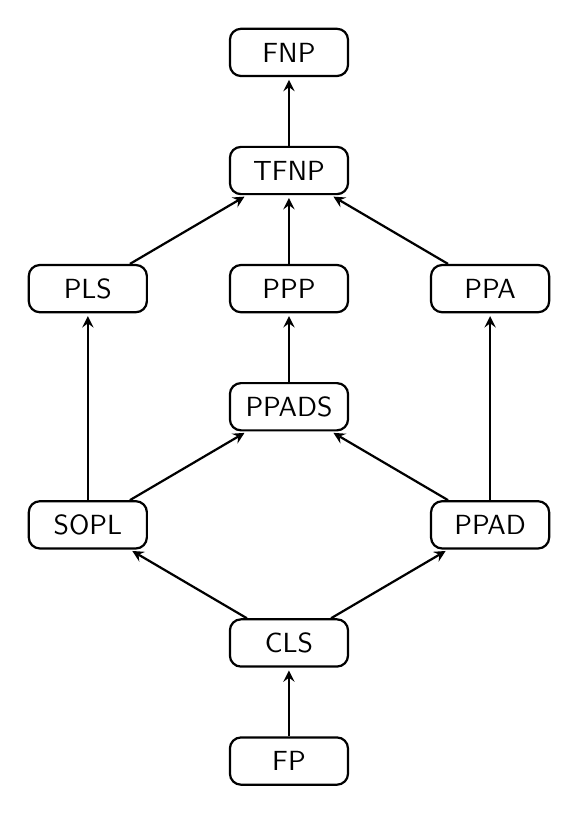
\begin{tikzpicture}[->,>=stealth,shorten >=1pt,auto,node distance=1.5cm, thick,main node/.style={scale=0.9,circle,draw,font=\sffamily\normalsize}]
    
        \node[rectangle, draw, rounded corners, minimum width=15mm, minimum height=6mm] (1) []{\textsf{FNP}};

        \node[rectangle, draw, rounded corners, minimum width=15mm, minimum height=6mm] (2) [below of = 1]{\textsf{TFNP}};

        \node[rectangle, draw, rounded corners, minimum width=15mm, minimum height=6mm] (3) [below of = 2]{\textsf{PPP}};

        \node[rectangle, draw, rounded corners, minimum width=15mm, minimum height=6mm] (4) [left of = 3, xshift=-30]{\textsf{PLS}};

        \node[rectangle, draw, rounded corners, minimum width=15mm, minimum height=6mm] (5) [right of = 3, xshift=30]{\textsf{PPA}};

        \node[rectangle, draw, rounded corners, minimum width=15mm, minimum height=6mm] (6) [below of = 3]{\textsf{PPADS}};

        \node (7) [below of = 6]{};

        \node[rectangle, draw, rounded corners, minimum width=15mm, minimum height=6mm] (8) [left of = 7, xshift=-30]{\textsf{SOPL}};

        \node[rectangle, draw, rounded corners, minimum width=15mm, minimum height=6mm] (9) [right of = 7, xshift=30]{\textsf{PPAD}};

        \node[rectangle, draw, rounded corners, minimum width=15mm, minimum height=6mm] (10) [below of = 7]{\textsf{CLS}};

        \node[rectangle, draw, rounded corners, minimum width=15mm, minimum height=6mm] (11) [below of = 10]{\textsf{FP}};
    
        \path[every node/.style={font=\sffamily\small}]
            (2) edge (1)
            (3) edge (2)
            (4) edge (2)
            (5) edge (2)
            (6) edge (3)
            (8) edge (4)
            (8) edge (6)
            (9) edge (5)
            (9) edge (6)
            (10) edge (8)
            (10) edge (9)
            (11) edge (10)
            ;
    \end{tikzpicture}
    
    \caption{Hierarchy of the main total search problem subclasses. \\ An arrow from class $A$ to class $B$ means that $A \subseteq B$.}
\end{figure}

Interestingly, lots of complex problems have been proven to be reducible to these basic problems. For example, the $\mathrm{NASH}$ problem relative to finding a Nash equilibrium of a given game has been shown to not only lie inside \textsf{PPAD} but also be \textsf{PPAD}-Complete \cite{nash_1, nash_2}. One should ponder what it really means for a problem to be complex.

Proving any unconditional separation between these subclasses, which can be achieved by showing that one of them is not efficiently reducible to the other, would directly imply that $\mathsf{FP} \neq \mathsf{TFNP}$, answering the $\mathsf{P} \stackrel{?}{=} \mathsf{NP}$. By the hardness of the question itself, finding such unconditional separation seems to be completely out of reach. However, it turns out that the \textsf{TFNP} model indeed has conditional separations, in particular relative to \textit{oracles} (see \Cref{chap:bb-tfnp}).
 
\newpage

\section{White-box \textsf{TFNP}}

In computer science and engineering, systems and models are divided into two categories: white-box systems and black-box systems. A system is said to be a \textbf{white-box} if its internal workings are known, meaning that given any input it is possible to know how the system achieves a result. Contrary, the computational process is unknown in a \textbf{black-box} system. Black-box models allow us to consider only the result for a given input, ignoring how that result is achieved. For example, a programmer uses both white-box and black-box systems: personal functions are white-boxes, while ready-to-go library functions are black-boxes.

Each \textsf{TFNP} problem can be analyzed through the lens of both white-box and black-box systems: in a \textbf{white-box \textsf{TFNP}} problem we're interested in how the problem gets verified (or solved if it's also in \textsf{FP}), while a \textbf{black-box \textsf{TFNP}} problem we're interested only in the verifiability (or computability) of the problem. Originally, these two models were characterized by solvability and verifiability through Turing machines \cite{decision_vs_search,rel_comp_np_search}. In recent years, researchers have shifted to another characterization: the white-box \textsf{TFNP} model is studied through \textit{protocols}, while black-box \textsf{TFNP} is studied through \textit{decision trees} \cite{separations_proof_complexity, adventures_monotone_tfnp, tfnp_characterization}. Any reader who has come this far will have asked himself the following question: why shift to other computational models? The answer is pretty straightforward: these two models are easier to work with. This shift of perspective allowed researchers to perform complex reasoning more easily, reaching otherwise unintuitive results. In this section, we will briefly discuss protocols and the white-box model, while decision trees and the black-box model will be extensively discussed in the following chapter. 

Suppose that we have two parties, namely Alice and Bob, who want to cooperate in order to achieve a common objective, like computing a function. To reach their goal, Alice and Bob must carry out separate computations, communicating the result to the other party in a pre-defined sequence of steps. This idea serves as groundwork for a definition of protocols, algorithms that dictate such alternations between computation and communications. 

We give the following formal definition of protocol. \cite{comm_compl_appl}

\begin{definition}
 Let $X$ be Alice's input set and let $Y$ be Bob's input set. A protocol $\pi$ is a rooted directed binary tree whose leaves are associated with outputs and internal nodes are owned by either Alice or Bob, where the owner of $v$ is noted by $\mathrm{owner}(v)$. Each leaf is labeled with an output $o \in O$, where $O$ is the outcome set. Each internal node $v$ is also associated to a function $g_v : Z \to \{0,1\}$, where $Z = X$ if $\mathrm{owner}(v) = \mathrm{A}$ and $Z = Y$ if $\mathrm{owner}(v) = \mathrm{B}$.
\end{definition}

When given the input $(x,y) \in X \times Y$, the protocol computes the associated function of the current node (starting from the root), proceeding on the left child if the output is 0 and on the right child if the output is 1. When a leaf is reached, the protocol returns the associated output. The output of the protocol for a given input $(x,y)$ is denoted with $\pi(x,y)$. A function $f$ is said to be computed by the protocol $\pi$ if for all inputs $(x,y)$ it holds that $f(x,y) = \pi(x,y)$.

\newpage

\begin{figure}[H]
    \centering

    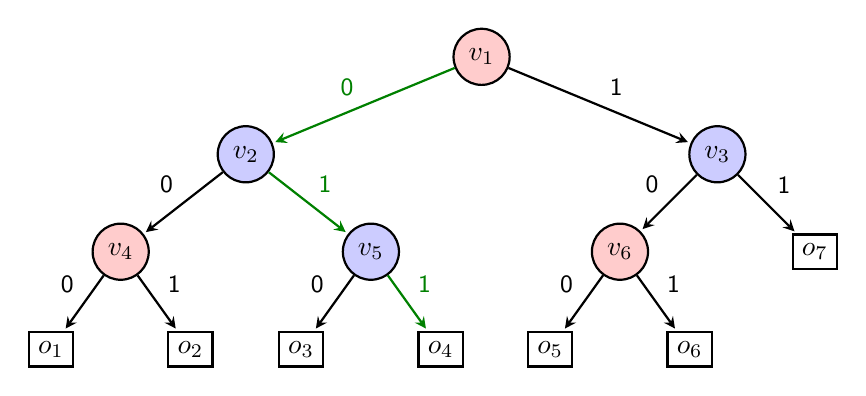
\begin{tikzpicture}[->,>=stealth,shorten >=1pt,auto,node distance=1.75cm, thick,main node/.style={scale=0.9,circle,draw,font=\sffamily\normalsize}]

        \node[circle, draw] (1)[fill=red!20] {$v_1$};

        \node[circle, draw] (2) [below left of=1, xshift=-50, fill=blue!20]{$v_2$};
        \node[circle, draw] (3) [below right of=1, xshift=50, fill=blue!20]{$v_3$};

        \node[circle, draw] (4) [below left of=2, xshift=-10, fill=red!20]{$v_4$};
        \node[circle, draw] (5) [below right of=2, xshift=10, fill=blue!20]{$v_5$};
        \node[circle, draw] (6) [below left of=3, fill=red!20]{$v_6$};
        \node[rectangle, draw] (7) [below right of=3]{$o_7$};

        \node[rectangle, draw] (8) [below left of=4, xshift=10]{$o_1$};
        \node[rectangle, draw] (9) [below right of=4, xshift=-10]{$o_2$};
        \node[rectangle, draw] (10) [below left of=5, xshift=10]{$o_3$};
        \node[rectangle, draw] (11) [below right of=5, xshift=-10]{$o_4$};
        \node[rectangle, draw] (12) [below left of=6, xshift=10]{$o_5$};
        \node[rectangle, draw] (13) [below right of=6, xshift=-10]{$o_6$};

        \path[every node/.style={font=\sffamily\small}]
 (1) edge[swap, color=Green]  node{0} (2)
 (1) edge node{1}(3)

 (2) edge[swap]  node{0} (4)
 (2) edge[color=Green]  node{1}(5)

 (3) edge[swap]  node{0} (6)
 (3) edge  node{1}(7)
            
 (4) edge[swap]  node{0} (8)
 (4) edge  node{1}(9)

 (5) edge[swap]  node{0} (10)
 (5) edge[color=Green]  node{1}(11)

 (6) edge[swap]  node{0} (12)
 (6) edge  node{1}(13)
 ;
    \end{tikzpicture}

    \caption{An example of a protocol of size 13 and depth 3 where the red nodes are owned by Alice and the blue nodes are owned by Bob. The green path shows the computation given by $f_{v_1}(x) = 0$, $f_{v_2}(y) = 1$ and $f_{v_5}(y) = 1$ for the input $(x,y)$}
\end{figure}

The complexity of protocols is measured in terms of their \textit{size} and \textit{depth}, that being the number of nodes of the protocol and the length of the longest directed path from the root node to a leaf. The \textbf{communication complexity} of a function $f$ is defined as the depth of the smallest protocol that computes $f$, corresponding to the minimal number of bits that must be communicated by Alice and Bob to compute $f$ for all possible inputs.

Protocols are clearly a Turing complete computational model: they are nothing more than an algorithm computed by two parties instead of one. Vice versa, a Turing machine can simulate a protocol by following the paths described by the protocol itself. This makes protocols a simple schematic way to define an algorithm. A protocol encodes all possible messages that may be sent by the parties during any conceivable conversation, producing the expected output. This means that a protocol always returns an answer for all possible inputs, making any function computed by a protocol \textit{total}. 

Furthermore, since the function processed by each step of the computation is explicitly defined and thus known, protocols are valid alternatives that characterize white-box \textsf{TFNP}. In particular, for each \textsf{TFNP} problem $R$, we denote with $R^{cc}$ the equivalent $\mathsf{TFNP}^{cc}$ problem, where \textit{cc} stands for \textit{communication complexity}. Due to them being defined on two inputs instead of one, communication search problems are defined on two sets of input values instead of one.

\begin{definition}
 A communication search problem is a sequence $R = (R_n)_{n \in \N}$ of relations $R_n \subseteq \{0,1\}^n \times \{0,1\}^n \times O_n$, one for each $n \in \N$, where each $O_n$ is a finite set called "outcome set".
\end{definition}

A protocol is considered to be efficient when its communication complexity is polylogarithmic with respect to the bit-size of the inputs, i.e. equal to $O(\log^k n)$. This ensures that there is a Turing machine capable of simulating the protocol in polynomial time. We give the following definitions of $\mathsf{FP}^{cc}$ and $\mathsf{FMP}^{cc}$

\begin{definition}
 We define $\mathsf{FP}^{cc}$ as the set of communication search problems $R = (R_n)_{n \in \N}$ for which there exists a polylogarithmic depth protocol $\pi_n$ such that $\pi_n(x,y) = z$ if and only if $((x,y), z) \in R_n$.
    \newpage
 We define $\mathsf{FNP}^{cc}$ as the set of communication search problems $R = (R_n)_{n \in \N}$ for which there exists a polylogarithmic depth protocol $V_n$ such that $V_n((x,y), z) = 1$ if and only if $((x,y), z) \in R_n$. 
\end{definition}

In this case, the certificate is the protocol itself: it defines a schema through which a Turing machine can verify the solution. The concept of reduction also applies to communication search problems, even though they require a pre-fixed value $t$ of the maximum amount of bits usable in the reduction, i.e. the maximum depth of the reduction protocol, which is necessary for computational reasons that we won't discuss. This allows us to define a $t$-bit \textsf{TFNP}$^{cc}$ hierarchy that follows the same structure as the standard one.

\begin{definition}
 A communication search problem $R = (R_m)_{m \in \N}$, where $R_m \subseteq \{0,1\}^m \times \{0,1\}^m \times O_m$, is said to be many-to-one reducible into a search problem $S = (S_n)_{n \in \N}$, where $S_n \subseteq \{0,1\}^n \times \{0,1\}^n \times O_n'$, if for all $m \in \N$ there is an $n \in \N$ for which there are two functions $f_X, f_Y : \{0,1\}^m \to \{0,1\}^n$ and a $t$-bit protocol $g : (\{0,1\}^m \times \{0,1\}^n) \times O_n' \to O_m$ such that:
    \[\forall (x,y) \in \{0,1\}^m \times \{0,1\}^m \;\; (f_X(x), f_Y(y), z) \in S \implies (x, y, \pi((x,y), z)) \in R\]
 In other words, the functions $f_X,f_Y$ map inputs of $R$ into inputs of $S$, while the protocol $g$ maps solutions of $S$ into solutions of $R$. 
\end{definition}

One of the most interesting properties of communication search problems is the ability to be characterized by a single type of search problem: the \textbf{monotone Karchmer-Widgerson game}. The game has a simple objective: given two inputs with different outputs, Alice and Bob have to cooperate to find a bit that differs between the two inputs.

\begin{definition}
 Given a Boolean function $f : \{0, 1\}^n \to \{0, 1\}$, we define the Karchmer-Wigderson game of $f$, denoted with $\mathrm{KW}(f)$, as the following communication problem: given the two inputs $x$ and $y$, where $f(x) = 0$ and $f(y) = 1$, find an index $i \in [n]$ such that $x_i \neq y_i$.

 If $f$ is a monotone Boolean function, meaning that given two inputs $x,y$ if $x \leq y$ then $f(x) \leq f(y)$, the monotone Karchmer-Widgerson game of $f$, denoted with $\mathrm{mKW}(f)$, finds an index $i \in [n]$ such that $x_i < y_i$.
\end{definition}

A surprising result \cite{span_programs, adventures_monotone_tfnp} proved that any communication search problem is equivalent to the monotone KW game of some Boolean function. This result implies that \textsf{TFNP}$^{cc}$ exactly is the study of the monotone Karchmer-Widgerson game.

\begin{lemma}
 For any communication search problem $R = (R_n)_{n \in \N}$, where $R_n \subseteq \{0,1\}^n \times \{0,1\}^n \times O_n$, in $t$-bit \textsf{TFNP}$^{cc}$, there is a function $f$ on $2^t\abs{O_n}$ variables such that $R$ is communication equivalent to $\mathrm{mKW}(f)$ under $t$-bit mapping reductions.
\end{lemma}

These games were originally introduced in 1990 by Karchmer and Widgerson \cite{kw_games} to show how the communication complexity of a game for a function $f$ is equal to the circuit complexity of a \textit{Boolean circuit} that solves the game on $f$.

\begin{theorem}
 Given a function $f : \{0, 1\}^n \to \{0, 1\}$, there is a circuit of depth $d$ that computes $f$ if and only if there is a protocol of depth $d$ that solves $\mathrm{KW}(f)$. Moreover, if $f$ is monotone, the circuit is monotone and the protocol solves $\mathrm{mKW}(f)$
\end{theorem}

In this case, Boolean circuits are defined as sets of logical AND and logical OR gates connected by cables. Like protocols, Boolean circuits have been proven to be Turing complete due to Turing machines and circuits being capable of simulating each other up to a polynomial factor \cite{sipser_computation}. Again, none should be dumbfounded by this result: any modern computer is just a large amount of Boolean gates wired together. We give the following definition of a Boolean circuit. \cite{comm_compl_appl}

\begin{definition}
 A Boolean circuit is a directed acyclic graph whose nodes, called gates, are associated with either input variables or Boolean operators. Each gate has an out-degree equal to 1 (except for the output gate which has out-degree 0) and in-degree equal to either 0 or 2. All 0 in-degree gates correspond to input variables, the negations of input variables or constant bits, while all 2 in-degree gates compute the logical AND or the logical OR of its given input variables or Boolean function. 
\end{definition}

Each gate $v$ is associated with the Boolean function $f_v$ computed by it. A function $f$ is said to be computer by a circuit with output gate $u$ if for all inputs $x \in \{0,1\}^n$ it holds that $f(x) =  f_u(x)$.

\begin{figure}[H]
    \centering

    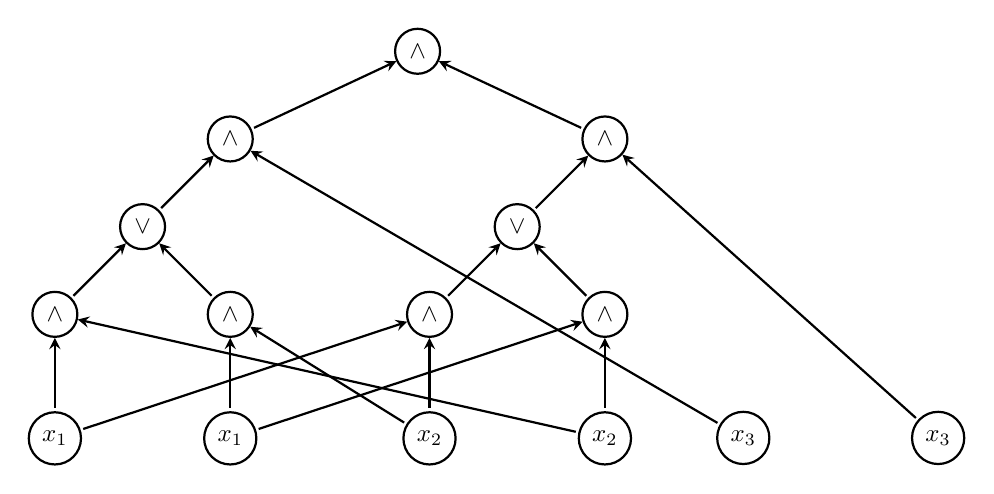
\begin{tikzpicture}[<-,>=stealth,shorten >=1pt,auto,node distance=1.75cm, thick,main node/.style={scale=0.9,circle,draw,font=\sffamily\normalsize}]

        \node[main node] (1) []{$\land$};

        \node[main node] (2) [below left of=1, xshift=-40]{$\land$};
        \node[main node] (3) [below right of=1, xshift=40]{$\land$};

        \node[main node] (4) [below left of=2]{$\lor$};
        \node[main node] (5) [below left of=4]{$\land$};
        \node[main node] (6) [below right of=4]{$\land$};
        \node[main node] (7) [below of=5]{$x_1$};
        \node[main node] (8) [below of=6]{$\vnot{x_1}$};

        \node[main node] (9) [below left of=3]{$\lor$};
        \node[main node] (10) [below left of=9]{$\land$};
        \node[main node] (11) [below right of=9]{$\land$};

        \node[main node] (12) [below of=10]{$x_2$};
        \node[main node] (13) [below of=11]{$\vnot{x_2}$};

        \node[] (14) [below right of=3, xshift=50]{};
        \node[] (15) [below left of=14]{};
        \node[] (16) [below right of=14]{};

        \node[main node] (17) [below of=15, yshift=8]{$x_3$};
        \node[main node] (18) [below of=16, yshift=8]{$\vnot{x_3}$};

        \path[every node/.style={font=\sffamily\small}]
            (1) edge (2)
            (1) edge (3)

            (2) edge (4) 
            (2) edge (17)

            (3) edge (9)
            (3) edge (18)

            (4) edge (5)
            (4) edge (6)

            (5) edge (7)
            (5) edge (13)

            (6) edge (8)
            (6) edge (12)

            (10) edge (7)
            (10) edge (12)

            (11) edge (8)
            (11) edge (13)

            (9) edge (10)
            (9) edge (11)

            ;
    \end{tikzpicture}

    \caption{A Boolean circuit of size 15 and depth 4 computing $x_1 \oplus x_2 \oplus x_3$.}
\end{figure}

The complexity of Boolean circuits is measured in terms of their \textit{size} and \textit{depth}, i.e. the number of gates of the circuit and the length of the longest directed path from an input gate to the output gate. However, differently from protocols, the \textbf{circuit complexity} of a function $f$ is defined as the size of the smallest Boolean circuit that computes it.

Karchmer and Widgerson's result allows us to characterize white-box \textsf{TFNP} in three ways: the study of communication search problems, the study of the monotone Karchmer-Widgerson game and the study of monotone Boolean circuits. This further extends the already known connections between search problems, communication complexity and circuit complexity, establishing that any result obtained in one of these fields can be in some way extended to the others.


\cleardoublepage